\documentclass{article}
\usepackage[utf8]{inputenc}

\usepackage[framed,numbered,autolinebreaks,useliterate]{mcode}
\usepackage{url}
\setlength{\parindent}{0pt}
\setlength{\parskip}{18pt}

\usepackage{graphicx}
\usepackage{amsmath}
\usepackage{amssymb}

\title{\textbf{Numerical Analysis – Winter 2021}}
\author{\textbf{3180100675}}
\date{2021.12.20}

\begin{document}

\maketitle

\section{Problem 1:}  
Refer to Lagrange interpolating polynomials definition, then: \\
\begin{equation}
\begin{aligned}
    P_2(x)&=f(x_0)L_{2,0}(x)+f(x_1)L_{2,1}(x)+f(x_2)L_{2,2}(x) \\
    &=f(x_0)\frac{(x-x_1)(x-x_2)}{(x_0-x_1)(x_0-x_2)}+f(x_1)\frac{(x-x_0)(x-x_2)}{(x_1-x_0)(x_1-x_2)}+f(x_2)\frac{(x-x_0)(x-x_1)}{(x_2-x_0)(x_2-x_1)} \nonumber
\end{aligned}
\end{equation}
To solve P1, i realize Lagrange interpolating polynomials in MATLAB, and Appendix A is its code, then i using it to construct these two function. Their results are as follow, and i also visualize their curves to ensure my solutions are right and compare them with the ground truth.

\textbf{Results and Error analysis}: \\
a.
According to f(x), $f^{(3)}(x)=-46\,\cos\left(3\,x\right)\,{\mathrm{e}}^{2\,x}-9\,\sin\left(3\,x\right)\,{\mathrm{e}}^{2\,x}$,
and because equation $f^{(4)}(x)=120\,\sin\left(3\,x\right)\,{\mathrm{e}}^{2\,x}-119\,\cos\left(3\,x\right)\,{\mathrm{e}}^{2\,x}=0$, root 0.2604 is among [0,0.6], which means the max number is $max(|f^{(3)}(0)|,|f^{(3)}(0.2604)|,|f^{(3)}(0.6)|)=max(46,65.6522,5.5999)=65.6522$, and to get the max peak of $g(x)=(x-0)(x-0.3)(x-0.6)$, $g^{'}(x)=3(x-0.1268)(x-0.4732)$, so the critical points occur at $max(|g(0.1268)|,|g(0.4732)|)=0.0104$. \\
Hence, the max absolute error is 
\begin{equation}
\begin{aligned}
    ERROR&=max|\frac{f^{(3)}(\partial)}{3!}| max|(x-0)(x-0.3)(x-0.6)|, x \in [0,0.6] \\
    &=\frac{65.6522 \times 0.0104}{3!} \\
    &=0.1138
    \nonumber
\end{aligned}
\end{equation}

\\
\begin{figure}
\centering
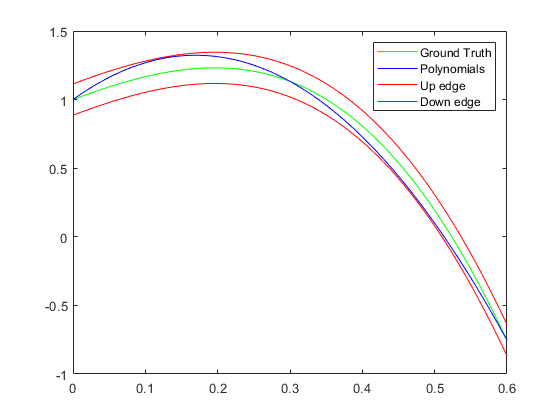
\includegraphics[width=7cm]{P1-a.png}
\caption{a. $\widetilde{f(x)}=1+3.808x-11.22x^2$}
\end{figure}

b.
According to f(x), $f^{(3)}(x)=\frac{\cos\left(\ln\left(x\right)\right)}{x^3}+\frac{3\,\sin\left(\ln\left(x\right)\right)}{x^3}$,
and because equation $f^{(4)}(x)=-\frac{10\,\sin\left(\ln\left(x\right)\right)}{x^4}=0$, there is no root among [2,2.6], which means the max number is $max(|f^{(3)}(2)|,|f^{(3)}(2.6)|)=max(0.3358,0.1722)=0.3358$, and to get the max peak of $g(x)=(x-2)(x-2.4)(x-2.6)$, $g^{'}(x)=3(x-2.1569)(x-2.5097)$, so the critical points occur at $max(|g(2.1569)|,|g(2.5097)|)=0.0169$. \\
Hence, the max absolute error is 
\begin{equation}
\begin{aligned}
    ERROR&=max|\frac{f^{(3)}(\partial)}{3!}| max|(x-2)(x-2.4)(x-2.6)|, x \in [2,2.6] \\
    &=\frac{0.3358 \times 0.0169}{3!} \\
    &=9.458 \times 10^{-4}
    \nonumber
\end{aligned}
\end{equation}

\begin{figure}[b]
\centering
\subfigure{
\begin{minipage}[t]{0.45\linewidth}
\centering
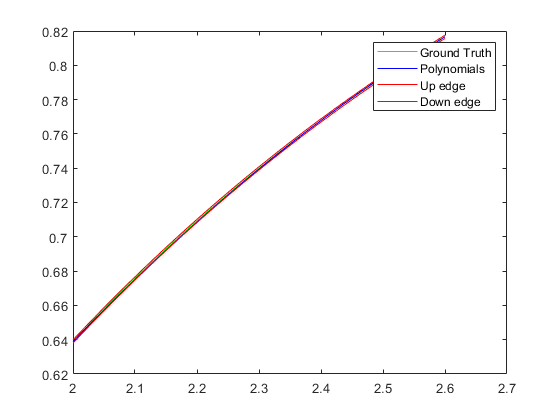
\includegraphics[width=6cm]{P1-b.png}
\end{minipage}%
}%
\subfigure{
\begin{minipage}[t]{0.45\linewidth}
\centering
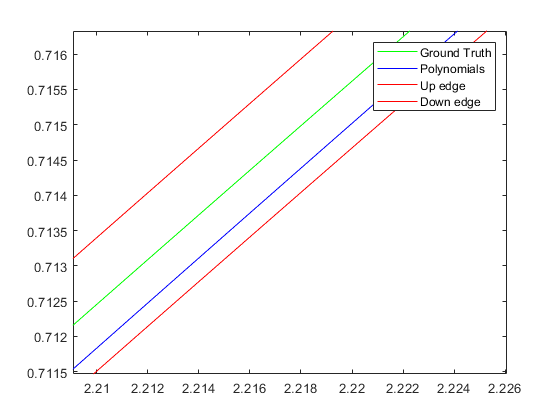
\includegraphics[width=6cm]{P1-b-local.png}
\end{minipage}%
}%
\caption{b. $\widetilde{f(x)}=-0.6325+0.8970x-0.1306x^2$}
\end{figure}

\section{Problem 2:}
Refer to interpolation formula: 
\begin{align*}
    P_3(x)&=0L_{3,0}(x)+y L_{3,1}(x)+3L_{3,2}(x)+2L_{3,3}(x) \\
    &=\frac{y(x-x_0)(x-x_2)(x-x_3)}{(x_1-x_0)(x_1-x_2)(x_1-x_3)} + \frac{3(x-x_0)(x-x_1)(x-x_3)}{(x_2-x_0)(x_2-x_1)(x_2-x_3)} + \frac{y(x-x_0)(x-x_1)(x-x_2)}{(x_3-x_0)(x_3-x_1)(x_3-x_2)}
    \\
    &\therefore \operatorname*{Coefficient}\limits_{x_{3}}P_3(x)=\frac{y}{0.5\times0.5\times1.5}+\frac{3}{-1\times0.5}+\frac{1}{1.5}=6 \\
    &\therefore y=\frac{17}{4}=4.25 \\
    \nonumber 
\end{align*}

\section{Problem 3:}
a. According to Neville's method, i inversely compute every element in the table: \\
Firstly, i compute $P_{0,1,2}$ by making good use of $P_{1,2,3}$ and $P_{0,1,2,3}$, that is: \\
\begin{equation}
\begin{aligned}
    P_{0,1,2,3} &= \frac{(x-x_0)P_{1,2,3}-(x-x_3)P_{0,1,2}}{x_3-x_0} \\
    &=\frac{1.4 \times 2.96+0.35 \times P_{0,1,2}}{0.75} \\
    &=3.016 \nonumber \\
\end{aligned}
\end{equation}
Finally i get $P_{0,1,2}=3.08$. \\
Following the same procedure above, it is easily to get all the missing entries: \\
$P_{0,1,2}=3.08$, $P_{1,2}=3.2$ and $P_{2}=f(0.5)=4$. \\

b. Apply the same method, below are my solutions: \\
\begin{equation}
\begin{aligned}
    P_{0,1,2}(x)&=\frac{(x-x_1)P_{0,2}(x)-(x-x_2)P_{0,1}(x)}{x_2-x_1} \\
             &=-x^2 + 3x + 1  \nonumber
\end{aligned}
\end{equation}
so $P_{0,1,2}(2.5)=2.25$, and then: \\
\begin{equation}
\begin{aligned}
    P_{0,1,2,3}(2.5)&=\frac{(x-x_0)P_{1,2,3}(2.5)-(x-x_3)P_{0,1,2}(2.5)}{x_3-x_0} \\
               &=2.875 \nonumber
\end{aligned}
\end{equation}

\section{Problem 4:} 
Following the backward propagation, it is obviously that: \\
\begin{equation}
    f[x_0,x_1,x_2]=\frac{f[x_1,x_2]-f[x_0,x_1]}{x_2-x_0}=\frac{10-f[x_0,x_1]}{0.7}=\frac{50}{7} \nonumber
\end{equation}
and then i get $f[x_0,x_1]=5$. \\
\begin{equation}
    f[x_1,x_2]=\frac{f[x_2]-f[x_1]}{x_2-x_1}=\frac{6-f[x_1]}{0.3}=10 \nonumber
\end{equation}
so $f[x_1]=3$, and \\
\begin{equation}
    f[x_0,x_1]=\frac{f[x_1]-f[x_0]}{x_1-x_0}=\frac{3-f[x_0]}{0.4}=5 \nonumber
\end{equation}
finally i get $f[x_0]=1$. \\


\section{Problem 5:}
Using cubic spline interpolating method, firstly i assume that:
\begin{equation}
\left\{  
\begin{array}{lr}
    S_0(x)=a_0+b_0x+c_0x^2+d_0x^3, & x \in [0,1] \\
    S_1(x)=a_1+b_1(x-1)+c_1(x-1)^2+d_1(x-1)^3, & x \in [1,2] \\
\end{array}
\right.
\end{equation}
and despite boundary conditions, we have: \\
\begin{equation}
\left\{  
\begin{array}{lr}
    S_0(0)=f(0)=0 \\
    S_0(1)=f(1)=1 \\
    S_1(1)=f(1)=1 \\
    S_1(2)=f(2)=2 \\
    S_0^{'}(1)=S_1^{'}(1) \\
    S_0^{''}(1)=S_1^{''}(1) \\
    \nonumber \\
\end{array}
\right.
\end{equation}
so substitute these number into equation (1), it will become: \\
\begin{equation}
\left\{  
\begin{array}{lr}
    a_0=0 \\
    a_0+b_0+c_0+d_0=1 \\
    a_1=1 \\
    a_1+b_1+c_1+d_1=2 \\
    b_0+2c_0+3d_0=b_1 \\
    c_0+3d_0=c_1 \\
    \nonumber \\
\end{array}
\right.
\end{equation}
Finally, align them with natural and clamped cubic spline conditions separately. \\
1. Natural cubic spline:
\begin{equation}
    S_0^{''}(0)=S_1^{''}(2)=0 \\
    \nonumber \\
\end{equation}
Solve the linear equations, then:
\begin{equation}
    S(x)=x, x \in [0,2] \nonumber
\end{equation}

2. Clamped cubic spline:
\begin{equation}
    S_0^{'}(0)=S_1^{'}(2)=1 \\
    \nonumber \\
\end{equation}
Solve the linear equations, then:
\begin{equation}
    S(x)=x, x \in [0,2] \nonumber
\end{equation}

\section{Problem 6:}
Assume strictly diagonally dominant matrix $A_{N \times N}$ is not invertible, then $A$ does not have full rank, so as to say its column vectors are linearly related, which means:\\
$\exists$ vector $v$, that $Av=0(v \neq 0)$, therefore in vector $v$, $\exists k, v_k=max(v) \neq 0$.
\begin{equation}
\begin{aligned}
    \because Av=0 
    \therefore \sum_{j=1}^N{a_{kj}v_j}=0 
    \therefore a_{kk}v_k=-\sum_{j=1, j \neq k}^N{a_{kj}{v_j}} 
    \therefore a_{kk}=-\sum_{j=1, j \neq k}^N{a_{kj}\frac{v_j}{v_k}} \\
    
    \centering 
    \therefore |a_{kk}| &=|\sum_{j=1, j \neq k}^N{a_{kj}\frac{v_j}{v_k}}| \\
    & \leq \sum_{j=1, j \neq k}^N{|a_{kj}| |\frac{v_j}{v_k}}| \\
    & \leq \sum_{j=1, j \neq k}^N{|a_{kj}|} \\
    \nonumber
\end{aligned}
\end{equation}
\\
\\
But due to strictly diagonally dominant matrix's definition: \\
\begin{equation}
    |a_{kk}| \geq \sum_{j=1, j \neq k}^N{|a_{kj}|} \nonumber \\
\end{equation}

So this leads to a contradiction, then my assumption is wrong, and original statement is proofed. 
\newpage
\appendix
\section{Appendix A}

\begin{lstlisting}
clc; clear; close all;
%% Main
main();
%% My functions
function main()
    % TODO, choose the Problem for solving
    problem = 1; % a
    % problem = 2; % b
    if (problem == 1) % a.
        x = [0, 0.3, 0.6];
        fx = exp(2. * x) .* cos(3 .* x);
    else % b.
        x = [2.0, 2.4, 2.6];
        fx = sin(log(x));
    end
    
    symf = lagrange_interpolte(x, fx);
    fprintf("Polynomials :\n");
    poly = matlabFunction(symf); disp(poly);
    X = linspace(x(1), x(end), 1000);
    if (problem == 1)
        Y = exp(2. * X) .* cos(3 .* X);
    else
        Y = sin(log(X));
    end
    polyY = poly(X);
    plot(X,Y,'color','g'); hold on;
    plot(X,polyY,'color','b'); hold on;
    if (problem == 1)
        ERR = 0.1138;
    else
        ERR = 0.0009458; 
    end
    upY = Y + ERR; downY = Y - ERR;
    plot(X,upY,'color','r'); hold on;
    plot(X,downY,'color','r'); hold on;
    legend("Ground Truth", "Polynomials", "Up edge", "Down edge");
end

function polynomials = lagrange_interpolte(X, Fx)
    n = size(X,2) - 1;
    syms x y;
    for i = 1 : n+1
        Xi = X; Xi(i) = [];
        if (i == 1)
            y = Fx(i) * prod(x - Xi) ./ prod(X(i) - Xi);
            continue;
        end
        y = y + Fx(i) * prod(x - Xi) ./ prod(X(i) - Xi);
    end
    y = simplify(y);
    polynomials = y;
end
\end{lstlisting}

\end{document}

